%
% introduction.tex
%
% Copyright The TTC 2.0 Contributors.
%
% TTC 2.0 Documentation
%
% This work is licensed under the Creative Commons Attribution-ShareAlike 4.0
% International License. To view a copy of this license,
% visit http://creativecommons.org/licenses/by-sa/4.0/.
%

%
% \brief Introduction chapter.
%
% \author Gabriel Mariano Marcelino <gabriel.mm8@gmail.com>
%
% \version 1.0.0
%
% \date 2021/04/01
%


\chapter{Introduction} \label{ch:introduction}

The TTC 2.0 is a Telemetry, Tracking and Command module designed for nanosatellites. It is one of the service modules developed for the GOLDS-UFSC CubeSat Mission \cite{floripasat2}, and part of the FloripaSat-2 platform \cite{marcelino2023}.

The module is a direct upgrade from the TTC of FloripaSat-1 \cite{ttc-fsat}, which grants a flight heritage rating. The improvements focus on providing a cleaner and more generic implementation than the previous version, more reliability in software and hardware implementations, and adaptations for the new mission requirements. All the project, source, and documentation files are available freely on a GitHub repository \cite{ttc2-repo} under the GPLv3 (firmware) and CERN OHLv2 (hardware) licenses.

\begin{figure}[!h]
	\begin{center}
		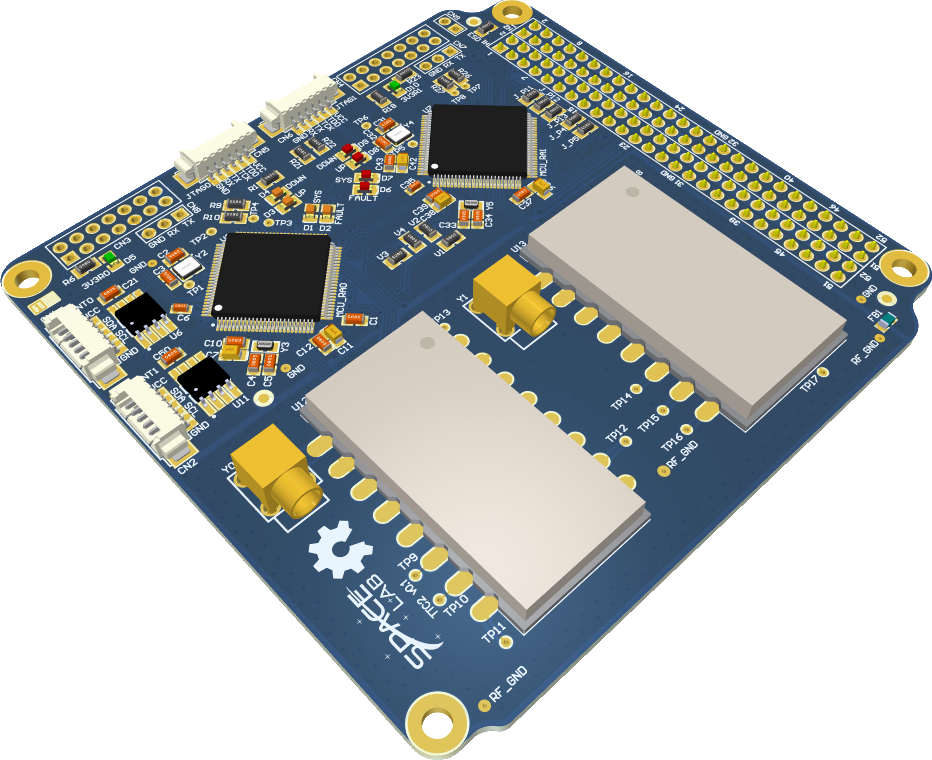
\includegraphics[width=0.65\textwidth]{figures/ttc2_pcb_3d.png}
		\caption{3D view of the TTC 2.0 PCB.}
		\label{fig:pcb-3d}
	\end{center}
\end{figure}

\section{Product tree}

The product tree of the TTC 2.0 module can be divided into three branches: hardware, firmware, and documentation. A diagram of the product tree is available in \autoref{fig:product-tree}.

\begin{figure}[!ht]
    \begin{center}
        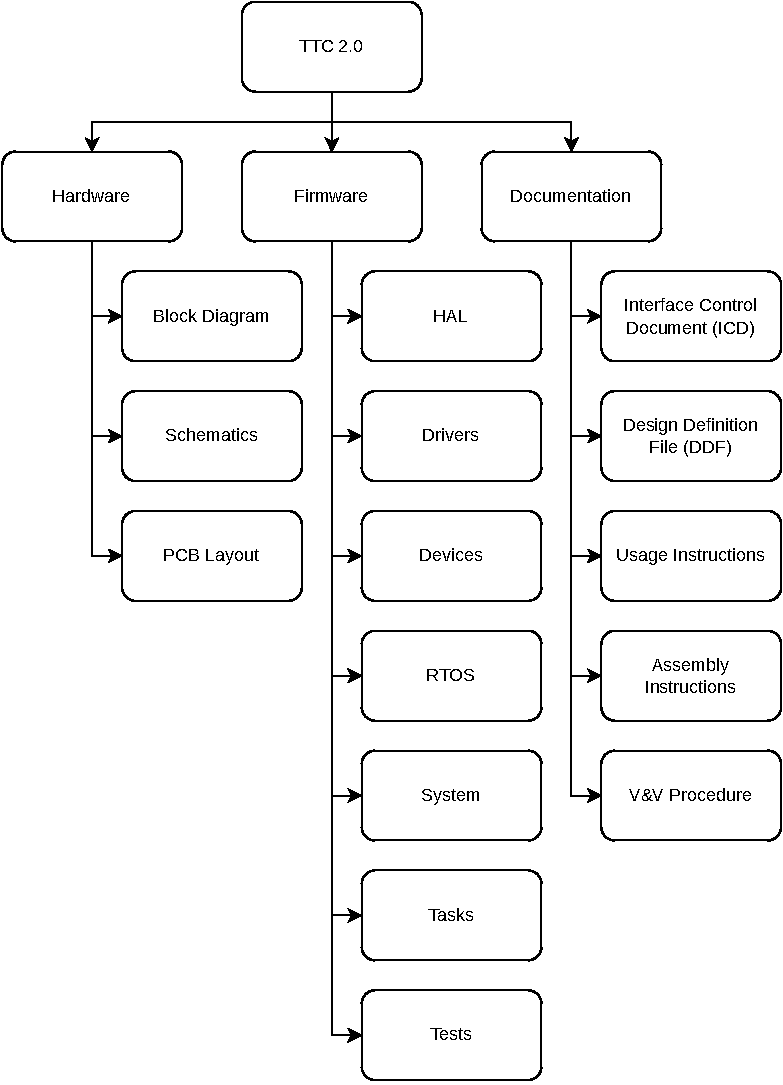
\includegraphics[width=0.8\textwidth]{figures/product-tree.pdf}
        \caption{Product tree of the TTC 2.0 module.}
        \label{fig:product-tree}
    \end{center}
\end{figure}

